\documentclass{beamer}
\usepackage[utf8]{inputenc}

\usetheme{Madrid}
\usecolortheme{default}
\usepackage{amsmath,amssymb,amsfonts,amsthm}
\usepackage{txfonts}
\usepackage{tkz-euclide}
\usepackage{listings}
\usepackage{adjustbox}
\usepackage{array}
\usepackage{tabularx}
\usepackage{gvv}
\usepackage{lmodern}
\usepackage{circuitikz}
\usepackage{tikz}
\usepackage{graphicx}

\setbeamertemplate{page number in head/foot}[totalframenumber]

\usepackage{tcolorbox}
\tcbuselibrary{minted,breakable,xparse,skins}

\definecolor{bg}{gray}{0.95}
\DeclareTCBListing{mintedbox}{O{}m!O{}}{%
breakable=true,
listing engine=minted,
listing only,
minted language=#2,
minted style=default,
minted options={%
linenos,
gobble=0,
breaklines=true,
breakafter=,,
fontsize=\small,
numbersep=8pt,
#1},
boxsep=0pt,
left skip=0pt,
right skip=0pt,
left=25pt,
right=0pt,
top=3pt,
bottom=3pt,
arc=5pt,
leftrule=0pt,
rightrule=0pt,
bottomrule=2pt,
toprule=2pt,
colback=bg,
colframe=orange!70,
enhanced,
overlay={%
\begin{tcbclipinterior}
\fill[orange!20!white] (frame.south west) rectangle ([xshift=20pt]frame.north west);
\end{tcbclipinterior}},
#3,
}
\lstset{
language=C,
basicstyle=\ttfamily\small,
keywordstyle=\color{blue},
stringstyle=\color{orange},
commentstyle=\color{green!60!black},
numbers=left,
numberstyle=\tiny\color{gray},
breaklines=true,
showstringspaces=false,
}

\title
{10.7.91}
\date{October 10, 2025}
\author
{EE25BTECH11043 - Nishid Khandagre}

\begin{document}

\frame{\titlepage}

\begin{frame}{Question}
The point of intersection of the tangents at the ends of the latus rectum of the parabola $y^2 = 4x$ is
\end{frame}

\begin{frame}{Solution}
The general form of a conic section is:
\begin{align}
\vec{x}^{\top}\vec{V}\vec{x} + 2\vec{u}^{\top}\vec{x} + f = 0
\end{align}
For the parabola $y^2 = 4x$, we can identify the matrices and vectors:
\begin{align}
\vec{V} &= \myvec{0 & 0 \\ 0 & 1} \\
\vec{u} &= \myvec{-2 \\ 0} \\
f &= 0
\end{align}
\end{frame}

\begin{frame}{Solution}
For a parabola $y^2 = 4ax$, the latus rectum endpoints are $(a, 2a)$ and $(a, -2a)$.

Given parabola is $y^2 = 4x$.
Comparing with $y^2 = 4ax$, we find $4a = 4$, which means $a=1$.

So, the endpoints of the latus rectum are:
\begin{align}
\vec{q_1} &= \myvec{1 \\ 2} \\
\vec{q_2} &= \myvec{1 \\ -2}
\end{align}
\end{frame}

\begin{frame}{Solution}
The tangent at a point $\vec{q}$ on the conic is given by the formula:
\begin{align}
\myvec{\vec{V}\vec{q} + \vec{u}}^{\top}\vec{x} + \vec{u}^{\top}\vec{q} + f = 0
\end{align}
Let's apply this for the first endpoint $\vec{q_1} = \myvec{1 \\ 2}$.
\end{frame}

\begin{frame}{Solution}
For $\vec{q_1} = \myvec{1 \\ 2}$:
\begin{align}
\vec{V}\vec{q_1} &= \myvec{0 & 0 \\ 0 & 1}\myvec{1 \\ 2} = \myvec{0\\ 2} \\
\vec{V}\vec{q_1} + \vec{u} &= \myvec{0 \\ 2} + \myvec{-2 \\ 0} = \myvec{-2 \\ 2} \\
\vec{u}^{\top}\vec{q_1} &= \myvec{-2 & 0}\myvec{1 \\ 2} = -2 \\
f &= 0
\end{align}
The tangent at $\vec{q_1}$ is:
\begin{align}
    \myvec{-2 \\ 2}^\top\vec{x} - 2 = 0\\
    \myvec{-1 \\ 1}^\top\vec{x}=1
    \end{align}
\end{frame}

\begin{frame}{Solution}
For $\vec{q_2} = \myvec{1 \\ -2}$:
\begin{align}
\vec{V}\vec{q_2} &= \myvec{0 & 0 \\ 0 & 1}\myvec{1 \\ -2} = \myvec{0 \\ -2} \\
\vec{V}\vec{q_2} + \vec{u} &= \myvec{0 \\ -2} + \myvec{-2 \\ 0} = \myvec{-2 \\ -2} \\
\vec{u}^{\top}\vec{q_2} &= \myvec{-2 & 0}\myvec{1 \\ -2} = -2 \\
f &= 0
\end{align}
The tangent at $\vec{q_2}$ is:
\begin{align}
    \myvec{-2 \\ -2}^\top\vec{x} - 2 = 0\\
    \myvec{1 \\ 1}^\top\vec{x}=-1
    \end{align}
\end{frame}

\begin{frame}{Solution}
    Intersection of the two tangents:
    \begin{align}
     \myvec{-1 \\ 1}^\top\vec{x}=1\\
    \myvec{1 \\ 1}^\top\vec{x}=-1\\
    \myvec{-1 & 1 \\ 1 & 1}\vec{x}=\myvec{1\\-1}
    \end{align}
   \begin{align}
   \myvec{
   -1 & 1 & \vrule & 1\\ 1 & 1 & \vrule & -1 
   }
   \end{align}
   $R_1\rightarrow -R_1$
   \begin{align}
   \myvec{
   1 & -1 & \vrule & -1\\ 1 & 1 & \vrule & -1 
   }\\
   \end{align}
\end{frame}
\end{frame}

\begin{frame}{Solution}
$R_2\rightarrow R_2-R_1$
   \begin{align}
   \myvec{
   1 & -1 & \vrule & -1\\ 0 & 2 & \vrule & 0
   }\\
   \end{align}
   $R_2\rightarrow R_2/2$, $R_1\rightarrow R_1+R_2$
   \begin{align}
   \myvec{
   1 & 0 & \vrule & -1\\ 0 & 1 & \vrule & 0
   }\\
   \vec{x}=\myvec{-1\\0}
   \end{align}
Therefore, the point of intersection is $\myvec{-1 \\ 0}$.
\end{frame}

\begin{frame}[fragile]
\frametitle{C Code}
\begin{lstlisting}[language=C]
#include <stdio.h>

// Function to find the point of intersection of tangents at the ends of the latus rectum
// For y^2 = 4ax, the ends of the latus rectum are (a, 2a) and (a, -2a)
// The tangents are:
// at (a, 2a): y(2a) = 2a(x + a)  => 2ay = 2ax + 2a^2 => y = x + a
// at (a, -2a): y(-2a) = 2a(x + a) => -2ay = 2ax + 2a^2 => -y = x + a => y = -x - a
//  x + a = -x - a => 2x = -2a => x = -a
// Substitute x = -a into y = x + a => y = -a + a => y = 0
void findIntersectionOfTangents(double a_param, double *intersect_x, double *intersect_y) {
    *intersect_x = -a_param;
    *intersect_y = 0.0;
}
\end{lstlisting}
\end{frame}

\begin{frame}[fragile]
\frametitle{Python Code through shared output}
\begin{lstlisting}[language=Python]
import ctypes
import numpy as np
import matplotlib.pyplot as plt

# Load the shared library
lib_code = ctypes.CDLL("/Users/nishidkhandagre/matgeo/venv/bin/code18.so")
# Define the argument types and return type for the C function
lib_code.findIntersectionOfTangents.argtypes = [
    ctypes.c_double,             # a_param
    ctypes.POINTER(ctypes.c_double), # intersect_x
    ctypes.POINTER(ctypes.c_double)  # intersect_y
]
lib_code.findIntersectionOfTangents.restype = None

# Given parabola: y^2 = 4x
# Comparing with y^2 = 4ax, we get 4a = 4, so a = 1
a_value = 1.0
\end{lstlisting}
\end{frame}

\begin{frame}[fragile]
\frametitle{Python Code through shared output}
\begin{lstlisting}[language=Python]
# Create ctypes doubles to hold the results
intersect_x_result = ctypes.c_double()
intersect_y_result = ctypes.c_double()

# Call the C function to find the point of intersection
lib_code.findIntersectionOfTangents(
    a_value,
    ctypes.byref(intersect_x_result),
    ctypes.byref(intersect_y_result)
)

intersection_x = intersect_x_result.value
intersection_y = intersect_y_result.value

print(f"For the parabola y^2 = 4x (where a = {a_value}):")
print(f"The point of intersection of the tangents at the ends of the latus rectum is ({intersection_x:.2f}, {intersection_y:.2f})")
\end{lstlisting}
\end{frame}

\begin{frame}[fragile]
\frametitle{Python Code through shared output}
\begin{lstlisting}[language=Python]
# --- Plotting Section ---
# Generate points for the parabola y^2 = 4x
y_parabola = np.linspace(-4, 4, 400)
x_parabola = (y_parabola**2) / 4

# Ends of the latus rectum
latus_rectum_end1_x, latus_rectum_end1_y = a_value, 2 * a_value
latus_rectum_end2_x, latus_rectum_end2_y = a_value, -2 * a_value

# Tangent equations derived from the problem (y = x + a and y = -x - a)
# For y = x + a (tangent at (a, 2a))
x_tangent1 = np.linspace(-3, 3, 100)
y_tangent1 = x_tangent1 + a_value

# For y = -x - a (tangent at (a, -2a))
x_tangent2 = np.linspace(-3, 3, 100)
y_tangent2 = -x_tangent2 - a_value
\end{lstlisting}
\end{frame}

\begin{frame}[fragile]
\frametitle{Python Code through shared output}
\begin{lstlisting}[language=Python]
plt.figure(figsize=(10, 8))

# Plot the parabola
plt.plot(x_parabola, y_parabola, 'b-', label='Parabola $y^2 = 4x$')
# Plot the focus
plt.scatter(a_value, 0, color='orange', s=100, zorder=5, label=f'Focus ({a_value}, 0)')
plt.annotate(f'F({a_value},0)', (a_value, 0), textcoords="offset points", xytext=(5,5), ha='left')
# Plot the latus rectum line
plt.plot([a_value, a_value], [-2*a_value, 2*a_value], 'k-', label='Latus Rectum (x=1)')

# Plot the ends of the latus rectum
plt.scatter(latus_rectum_end1_x, latus_rectum_end1_y, color='red', s=100, zorder=5, label=f'End L ({latus_rectum_end1_x},{latus_rectum_end1_y})')
\end{lstlisting}
\end{frame}

\begin{frame}[fragile]
\frametitle{Python Code through shared output}
\begin{lstlisting}[language=Python]
plt.annotate(f'L({latus_rectum_end1_x},{latus_rectum_end1_y})', (latus_rectum_end1_x, latus_rectum_end1_y), textcoords="offset points", xytext=(5,5), ha='left')
plt.scatter(latus_rectum_end2_x, latus_rectum_end2_y, color='red', s=100, zorder=5, label=f'End L\' ({latus_rectum_end2_x},{latus_rectum_end2_y})')
plt.annotate(f'L\'({latus_rectum_end2_x},{latus_rectum_end2_y})', (latus_rectum_end2_x, latus_rectum_end2_y), textcoords="offset points", xytext=(5,5), ha='right')

# Plot the tangents
plt.plot(x_tangent1, y_tangent1, 'g-', label=f'Tangent at L (y=x+{a_value})')
plt.plot(x_tangent2, y_tangent2, 'm-', label=f'Tangent at L\' (y=-x-{a_value})')
\end{lstlisting}
\end{frame}

\begin{frame}[fragile]
\frametitle{Python Code through shared output}
\begin{lstlisting}[language=Python]
# Plot the intersection point
plt.scatter(intersection_x, intersection_y, color='purple', s=100, zorder=6, label=f'Intersection ({intersection_x:.2f},{intersection_y:.2f})')
plt.annotate(f'P({intersection_x:.2f},{intersection_y:.2f})', (intersection_x, intersection_y), textcoords="offset points", xytext=(10, -15), ha='left', color='purple', fontsize=12)
plt.xlim(-3, 6)
plt.ylim(-4, 4)
plt.gca().set_aspect('equal', adjustable='box')
plt.xlabel('X-axis')
plt.ylabel('Y-axis')
plt.title('Parabola, Latus Rectum, Tangents, and Intersection Point')
plt.grid(True)
plt.legend()
plt.axhline(0, color='gray', linewidth=0.5)
plt.axvline(0, color='gray', linewidth=0.5)
plt.show()
\end{lstlisting}
\end{frame}

\begin{frame}[fragile]
\frametitle{Python Code : Direct}
\begin{lstlisting}[language=Python]
import numpy as np
import matplotlib.pyplot as plt

def find_intersection_of_tangents_at_latus_rectum_ends(a_param):
    #the ends of the latus rectum are:
    # L1 = (a, 2a)
    # L2 = (a, -2a)
    # 2. Determine the equations of the tangents at these points
    # The general equation of a tangent to y^2 = 4ax at a point (x1, y1) is:
    # y * y1 = 2a * (x + x1)
    # Tangent at L1 (a, 2a):
    # y * (2a) = 2a * (x + a)
    # y = x + a  (Equation for Tangent 1)

    # Tangent at L2 (a, -2a):
    # y * (-2a) = 2a * (x + a)
    # y = -x - a (Equation for Tangent 2)
\end{lstlisting}
\end{frame}

\begin{frame}[fragile]
\frametitle{Python Code : Direct}
\begin{lstlisting}[language=Python]
    # Solving the system:
    # x + a = -x - a
    # x = -a

    # Substitute x = -a
    # y = (-a) + a
    # y = 0

    x_intersect = -a_param
    y_intersect = 0.0
    return x_intersect, y_intersect

# --- Main execution and plotting ---
# Given parabola: y^2 = 4x
# 4a = 4  => a = 1
a_value = 1.0
\end{lstlisting}
\end{frame}

\begin{frame}[fragile]
\frametitle{Python Code : Direct}
\begin{lstlisting}[language=Python]
# Calculate the intersection point using the Python function
intersection_x, intersection_y = find_intersection_of_tangents_at_latus_rectum_ends(a_value)

print(f"For the parabola y^2 = 4x (where a = {a_value}):")
print(f"The point of intersection of the tangents at the ends of the latus rectum is ({intersection_x:.2f}, {intersection_y:.2f})")

# --- Plotting Section ---
plt.figure(figsize=(10, 8))

# 1. Plot the parabola y^2 = 4x
y_parabola = np.linspace(-4, 4, 400)
x_parabola = (y_parabola**2) / (4 * a_value)
plt.plot(x_parabola, y_parabola, 'b-', label=f'Parabola $y^2 = 4x$')
\end{lstlisting}
\end{frame}

\begin{frame}[fragile]
\frametitle{Python Code : Direct}
\begin{lstlisting}[language=Python]
# 2. Plot the focus
focus_x, focus_y = a_value, 0
plt.scatter(focus_x, focus_y, color='orange', s=100, zorder=5, label=f'Focus ({focus_x}, {focus_y})')
plt.annotate(f'F({focus_x},{focus_y})', (focus_x, focus_y), textcoords="offset points", xytext=(5,5), ha='left')

# 3. Plot the latus rectum line
latus_rectum_x_val = a_value
latus_rectum_y_min, latus_rectum_y_max = -2 * a_value, 2 * a_value
plt.plot([latus_rectum_x_val, latus_rectum_x_val], [latus_rectum_y_min, latus_rectum_y_max], 'k-', label='Latus Rectum (x=1)')
\end{lstlisting}
\end{frame}

\begin{frame}[fragile]
\frametitle{Python Code : Direct}
\begin{lstlisting}[language=Python]
# 4. Plot the ends of the latus rectum
latus_rectum_end1 = (a_value, 2 * a_value)
latus_rectum_end2 = (a_value, -2 * a_value)
plt.scatter(latus_rectum_end1[0], latus_rectum_end1[1], color='red', s=100, zorder=5, label=f'End L ({latus_rectum_end1[0]},{latus_rectum_end1[1]})')
plt.annotate(f'L({latus_rectum_end1[0]},{latus_rectum_end1[1]})', latus_rectum_end1, textcoords="offset points", xytext=(5,5), ha='left')
plt.scatter(latus_rectum_end2[0], latus_rectum_end2[1], color='red', s=100, zorder=5, label=f'End L\' ({latus_rectum_end2[0]},{latus_rectum_end2[1]})')
plt.annotate(f'L\'({latus_rectum_end2[0]},{latus_rectum_end2[1]})', latus_rectum_end2, textcoords="offset points", xytext=(5,-5), ha='right')
\end{lstlisting}
\end{frame}

\begin{frame}[fragile]
\frametitle{Python Code : Direct}
\begin{lstlisting}[language=Python]
# 5. Plot the tangents
x_tangent_range = np.linspace(-3, 3, 100)
y_tangent1 = x_tangent_range + a_value
y_tangent2 = -x_tangent_range - a_value

plt.plot(x_tangent_range, y_tangent1, 'g-', label=f'Tangent at L (y=x+{a_value})')
plt.plot(x_tangent_range, y_tangent2, 'm-', label=f'Tangent at L\' (y=-x-{a_value})')

# 6. Plot the intersection point
plt.scatter(intersection_x, intersection_y, color='purple', s=100, zorder=6, label=f'Intersection ({intersection_x:.2f},{intersection_y:.2f})')
plt.annotate(f'P({intersection_x:.2f},{intersection_y:.2f})', (intersection_x, intersection_y), textcoords="offset points", xytext=(10, -15), ha='left', color='purple', fontsize=12)
\end{lstlisting}
\end{frame}

\begin{frame}[fragile]
\frametitle{Python Code : Direct}
\begin{lstlisting}[language=Python]
# --- Plot Aesthetics ---
plt.xlim(-3, 6)
plt.ylim(-4, 4)
plt.gca().set_aspect('equal', adjustable='box')
plt.xlabel('X-axis')
plt.ylabel('Y-axis')
plt.title('Parabola, Latus Rectum, Tangents, and Intersection Point')
plt.grid(True)
plt.legend()
plt.axhline(0, color='gray', linewidth=0.5)
plt.axvline(0, color='gray', linewidth=0.5)
plt.show()
\end{lstlisting}
\end{frame}

\begin{frame}
\begin{figure}[H]
\centering
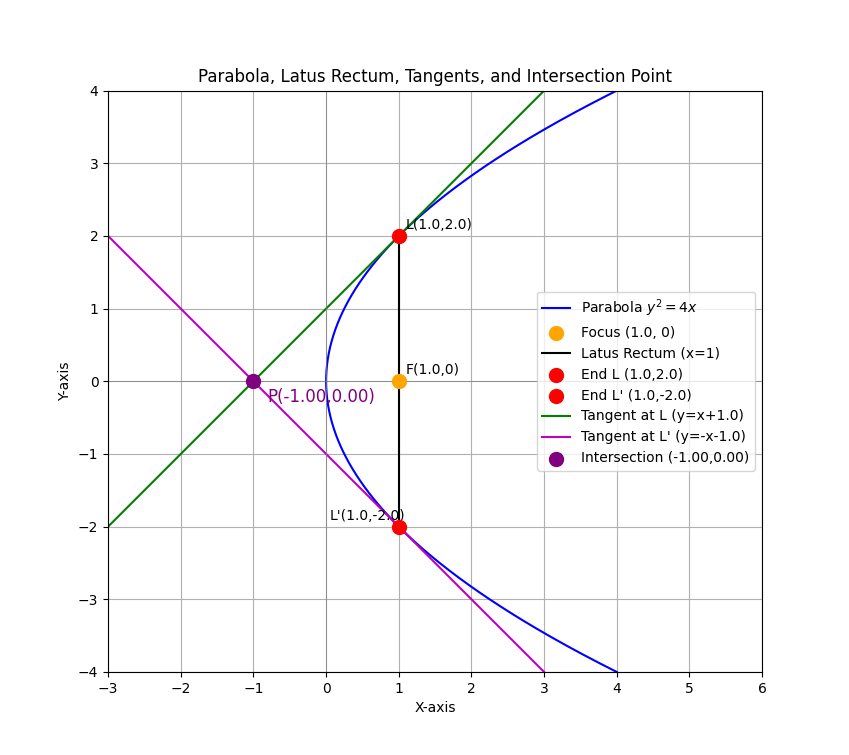
\includegraphics[width=0.8\columnwidth]{../figs/mat181.png}
\caption{}
\label{fig:1}
\end{figure}
\end{frame}

\begin{frame}
\begin{figure}[H]
\centering
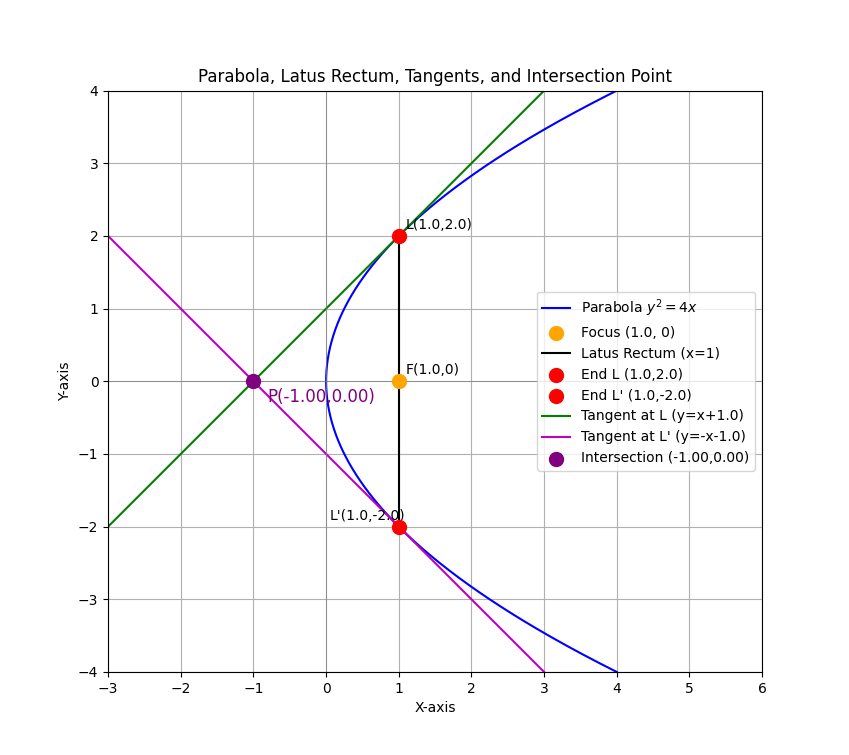
\includegraphics[width=0.7\columnwidth]{../figs/mat181.png}
\caption{}
\label{fig:2}
\end{figure}
\end{frame}

\end{document}
